\documentclass[tikz]{standalone}
\usepackage{tikz}
\usetikzlibrary{positioning, graphs}
\usetikzlibrary{graphs.standard}
\begin{document}
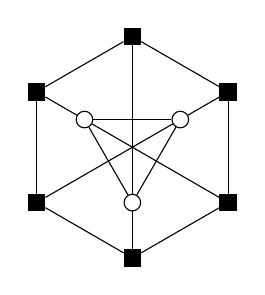
\begin{tikzpicture}
        \graph[clockwise, radius = 4em, phase = 30, empty nodes,
            nodes={rectangle, draw, inner sep = 0, minimum size = 0.6em, fill=black}]
                {subgraph C_n[n = 6, name = A]};
        \graph[clockwise, radius = 2em, phase = 30, empty nodes,
            nodes={circle, draw, inner sep = 0, minimum size = 0.6em}]
                {subgraph C_n[n = 3, name = B]};
        
        \draw (B 1) -- (A 1);
        \draw (B 1) -- (A 4);
        \draw (B 2) -- (A 3);
        \draw (B 2) -- (A 6);
        \draw (B 3) -- (A 2);
        \draw (B 3) -- (A 5);
\end{tikzpicture}
\end{document}